\documentclass[10pt,a4paper]{article}
\usepackage[margin=1.6cm]{geometry}
\usepackage[latin1]{inputenc}
\usepackage{amsmath}
\usepackage{amsfonts}
\usepackage{amssymb}
\usepackage{multirow}
\usepackage{graphicx}
\usepackage{subcaption}
\author{Hector Dearman \and Paul Rowe-White \and Kritaphat Songsriin \and Simon Stuckemann}
\title{Machine Learning CBC: Decision Trees}
\begin{document}
\maketitle

\section{Implementation Summary}

In order to gather statistical results of our algorithm and compare the performance of different approaches we implemented a few functions that would help us with this task.

To perform 10-fold cross validation efficiently we implemented the function \texttt{cross\_fold \_validation(x, y)} (Figure~\ref{fig:cross_fold_validation}) which takes examples \texttt{x} and classifications \texttt{y} and returns a confusion matrix that was found by performing several tests using 10-fold cross validation. In this function, the set of examples are split into 10 folds using function {\tt create\_folds(10, x, y)}(Figure~\ref{fig:create_folds}), leaving out any extra examples so that each fold is of the same size. In 10 iterations the algorithm then removes one of the buckets as the test set and combines the rest into a training set (no validation set is required in this part of the coursework).The training set is then used to train a decision tree using the \texttt{build\_tree(training\_data\_x, training\_data\_y, attribute)}(Figure~\ref{fig:build_tree}) which build the decision tree for the given attribute using the given data (consisting of 9 folds). The given {\tt training\_data\_y} is converted into a vector of binary target using function {\tt binary\_filter}(Figure~\ref{fig:binary_filter}). The function then tests the trees using the \texttt{test\_trees} function(Figure~\ref{fig:test_trees}) which returns a vector of predictions by calling function {\tt test\_tree}(Figure~\ref{fig:test_tree}) for each tree. If there are more than one tree that return true, an aprropiate algorithm(first positive, random positive, or shortest path) will be applied. The predictions are then compared to the actual classifications and the results are added to a confusion matrix. After all values have been added from all ten folds the confusion matrix is turned into an average confusion matrix by simply dividing the values by 10 and returned to the user. 

Note that this means that any error rate or other statistics given in this report is based on the average confusion matrix and not given in terms of the average of many calculations of that statistic over the course of the cross validation.
% elaborate here?

As part of the \texttt{build\_tree} function we implemented a function that selects the best attribute from a set of attributes on which to split the set of examples. This function (\texttt{choose\-\_best\-\_decision\-\_attribute(examples, attributes, binary\_targets)} in Figure~\ref{fig:choose_best_decision_attribute}) maximises the information gain of each possible split and thus returns the attribute that returns the largest information gain (n = negative examples, p = positive examples, $p_0$ = positive examples of the subset of data for which the attribute has a value 0, etc.):

\begin{align}
Gain(attribute)  &= I(p,n) - Remainder(attribute)\\
I(p,n) &= -\left(\frac{p}{p+n}\right)\log_2{\left(\frac{p}{p+n}\right)} -\left(\frac{n}{p+n}\right)\log_2{\left(\frac{n}{p+n}\right)}\\
Remainder(attribute) &= \frac{p_0 + n_0}{p+n}I(p_0,n_0) + \frac{p_1 + n_1}{p + n}I(p_1,n_1)
\end{align}
Note that in the implementation of $I(p,n)$ in Figure~\ref{fig:entropy} we check explicitly for the case when $p = 0$ or $n = 0$ as Matlab will otherwise return $NaN$ which will result in unbalanced trees. Also, for performance reasons we do not actually calculate the information gain but instead simply return the minimum value of the remainder(Figure~\ref{fig:remainder}).
%Hector: maybe say we don't calculate gain for performance reasons, instead we just use the min of remainder?
%elaborate here maybe?


\section{Diagrams of six trees}
See Figure~\ref{fig:tree1}, Figure~\ref{fig:tree2}, Figure~\ref{fig:tree3}, Figure~\ref{fig:tree4}, Figure~\ref{fig:tree5} and Figure~\ref{fig:tree6}


\section{Evaluation}
\subsection{Clean Dataset}
Analysis of the clean dataset results in the confusion matrix that can be seen in table \ref{tab:chooseDepthCleanConfusion}. From this confusion matrix, the recall and precision rates can be calculated which can then be combined to a single $F_1$ measure as seen in table \ref{tab:chooseDepthCleanStats}.
\begin{table}[!ht]
\centering
\begin{tabular}{|l|c|c|c|c|c|c|c|}
	\cline{3-8}
	\multicolumn{2}{c}{}& \multicolumn{6}{ |c| }{Predicted class}\\
	\cline{3-8}
	\multicolumn{2}{c|}{} & 1 & 2 & 3 & 4 & 5 & 6\\ \cline{1-8}
	\multirow{6}{*}{Actual class}& 1 & 8.4 & 1.8 & 0.6 & 0.4 & 1.5 & 0.4 \\ \cline{2-8}
	& 2 & 1.8 & 14.7 & 0.3 & 1.0 & 1.3 & 0.7\\ \cline{2-8}
	& 3 & 0.4 & 0.6 & 8.6 & 0.4 & 0.3 & 1.5 \\ \cline{2-8}
	& 4 & 0.1 & 1.1 & 0.3 & 18.1 & 1.4 & 0.5 \\ \cline{2-8}
	& 5 & 1.7 & 1.4 & 0.4 & 0.8 & 8.1 & 0.8 \\ \cline{2-8}
	& 6 & 0 & 0.5 & 1.5 & 0.6 & 0.9 & 17.1\\ \hline
\end{tabular}
\caption{Confusion Matrix of Final Algorithm Applied to Clean Data}
\label{tab:chooseDepthCleanConfusion}
\end{table}


\begin{table}[!ht]
\centering
\begin{tabular}{|l|c|c|c|c|c|c|}
	\cline{2-7}
	\multicolumn{1}{c|}{}& \multicolumn{6}{ |c| }{Class}\\
	\cline{2-7}
	\multicolumn{1}{c|}{}& 1 & 2 & 3 & 4 & 5 & 6\\ \hline
	Recall Rate & 64.1221 & 74.2424 & 72.8814 & 84.1860 & 61.3636 & 83.0097\\ \hline
	Precision Rate & 67.7419 & 73.1343 & 73.5043 & 84.9765 & 60.0000 & 81.4286\\ \hline
	$F_1$ & 65.8824 & 73.6842 & 73.1915 & 84.5794 & 60.6742 & 82.2115\\ \hline
\end{tabular}
\caption{Statistics for Final Algorithm Applied to Clean Data}
\label{tab:chooseDepthCleanStats}
\end{table}

In addition, the calculated error rate is $0.2500$, resulting in a classification rate of $0.7500$ (see table \ref{tab:chooseDepthRates}).

\subsection{Noisy Dataset}

Analysis of the noisy dataset results in the confusion matrix that can be seen in table \ref{tab:chooseDepthNoisyConfusion}. From this confusion matrix, the recall and precision rates can be calculated which can then be combined to a single $F_1$ measure as seen in table \ref{tab:chooseDepthNoisyStats}.

\begin{table}[!ht]
\centering
\begin{tabular}{|l|c|c|c|c|c|c|c|}
	\cline{3-8}
	\multicolumn{2}{c}{}& \multicolumn{6}{ |c| }{Predicted class}\\
	\cline{3-8}
	\multicolumn{2}{c|}{}  & 1 & 2 & 3 & 4 & 5 & 6\\ \cline{1-8}
	\multirow{7}{*}{Actual class} & 1 & 3.1 & 0.7 & 1.7 & 0.8 & 1.9 & 0.6 \\ \cline{2-8}
	& 2 & 1.6 & 12.3 & 2.2 & 1.5 & 0.8 & 0.3\\ \cline{2-8}
	& 3 & 1.4 & 1.7 & 10.6 & 2.3 & 1.0 & 1.7 \\ \cline{2-8}
	& 4 & 0.8 & 1.1 & 1.4 & 15.7 & 0.5 & 1.3 \\ \cline{2-8}
	& 5 & 2.0 & 0.8 & 0.8 & 0.7 & 5.8 & 0.9 \\ \cline{2-8}
	& 6 & 1.1 & 0.4 & 2.0 & 0.8 & 1.1 & 16.6\\ \hline
\end{tabular}
\caption{Confusion Matrix of Final Algorithm Applied to Noisy Data}
\label{tab:chooseDepthNoisyConfusion}
\end{table}

\begin{table}
\centering
\begin{tabular}{|l|c|c|c|c|c|c|}
	\hline
	& \multicolumn{6}{ |c| }{Class}\\
	\hline
	& 1 & 2 & 3 & 4 & 5 & 6\\ \hline
	Recall Rate & 35.2273 & 65.7754 & 56.6845 & 75.4808 & 52.7273 & 75.4545 \\ \hline
	Precision Rate & 31.0000 & 72.3529 & 56.6845 & 72.0183 & 52.2523 & 77.5701\\ \hline
	$F_1$ & 32.9787 & 68.9076 & 56.6845 & 73.7089 & 52.4887 & 76.4977\\ \hline
\end{tabular}
\caption{Statistics for Final Algorithm Applied to Noisy Data}
\label{tab:chooseDepthNoisyStats}
\end{table}

In addition, the calculated error rate is $0.3590$, resulting in a classification rate of $0.6410$ (see table \ref{tab:chooseDepthRates}).

\subsection{Conclusion}

There is a difference in the performance when using the clean and noisy datasets. The clean set performs a lot better than the other. This is because while the clean dataset contains only consistent classifications, the noisy set also contains examples with their classifications that do not agree. Because of this, the trees that are constructed from this data classify examples incorrectly.


\section{Emotion Ambiguity}

During the training phase six decision trees are built, each corresponding to one of the six emotions \emph{Happiness}, \emph{Sadness}, \emph{Surprise}, \emph{Disgust}, \emph{Fear}, and \emph{Anger}. When the decision trees are then used to determine whether a given example is an example of either of these emotions it is possible that more than of the trees classifies the example positively, thus making the outcome ambiguous, since the example could now indicate multiple emotions. 

In order to return one of the emotions to the end user the algorithm needs to pick one of the positive emotions (or indeed one of the negative if none of the trees classified the example positively). To find out which approach leads to the best result we tried to use multiple algorithms and compared their performance.

\subsection{Choose First Positive Classification}

A very simple solution to the problem and arguably the easiest to implement is to always select the first positively classified emotion, or indeed the first emotion if none of the classifiers returned a positive result. In \emph{Matlab} this can be implemented by simply using the \texttt{max} function on the row vector of results. Simplicity is the main advantage of this approach: the code that implements this solution not only is easy to read but also is one of the fastest mechanisms to decide between different solutions. However, this approach also has many disadvantages. For instance, there is no inherent order in the emotions, which means that the trees corresponding to the emotions can also not be ordered. Always choosing the first occurrence of a positive classification thus seems arbitrary and results in a large skew of the distribution of classifications.

This disadvantage also shows in the statistical evaluation of this approach as we can see in tables \ref{tab:chooseFirstStats} and \ref{tab:chooseFirstRates}. It can clearly be seen that there is again a difference between the clean and noisy datasets. This is consistent with the end results discussed above and (briefly) below. It can be seen that the error rate is $27.2\%$ is relatively large for clean data. However, in noisy data the performance of this approach drops significantly to an error rate of $40.7\%$. A closer look at the individual recall and precision rates in table \ref{tab:chooseFirstStats} explains why: The precision rate, which measures the number of false positives, is extremely low with only $19.29\%$ ($F_1 = 29.65\%$) in the first classifier for the noisy data set which can be explained by the favouritism in this approach. It is also apparent that the number of false negatives (as measured by the recall rate) is is relatively large in all other classes, which can also  be explained by the skew.

\begin{table}
\centering
\begin{tabular}{|l|c|c|c|c|c|c|}
	\hline
	& \multicolumn{6}{ |c| }{Class}\\
	\hline
	& 1 & 2 & 3 & 4 & 5 & 6\\ \hline
	Recall Rate Clean & 83.9695 & 73.2323 & 66.9492 & 81.3953 & 49.2424 & 74.7573 \\ \hline
	Precision Rate Clean & 42.8016 & 76.7196 & 77.4510 & 90.2062 & 73.0337 & 91.1243\\ \hline
	$F_1$ Clean & 56.7010 & 74.9354 & 71.8182 & 85.5746 & 58.8235 & 82.1333\\ \hline \hline
	Recall Rate Noisy & 55.6818 & 67.9144 & 52.4064 & 66.8269 & 40.0000 & 61.8182 \\ \hline
	Precision Rate Noisy & 19.2913 & 71.7514 & 62.4204 & 78.9773 & 61.1111 & 82.9268\\ \hline
	$F_1$ Noisy & 28.6550 & 69.7802 & 56.9767 & 72.3958 & 48.3516 & 70.8333\\ \hline
\end{tabular}
\caption{Statistics for \emph{Choose-First} Algorithm}
\label{tab:chooseFirstStats}
\end{table}

\begin{table}[!ht]
\centering
\begin{tabular}{|c|c|c|}
\hline 
 & \textbf{Error Rate} & \textbf{Classification Rate} \\ 
\hline 
Clean Data & $0.2720$ & $0.7280$ \\ 
\hline 
Noisy Data & $0.4070$ & $0.5930$ \\ 
\hline 
\end{tabular} 
\caption{Error Rate and Classification Rate in \emph{Choose-First} Algorithm}
\label{tab:chooseFirstRates}
\end{table}

\subsection{Choose Random Positive Classification}
One way to avoid the skew that we encountered in the previous approach is to choose a random positive classification from the set of positive classifications using a uniform distribution. The advantage of this approach is that it is also relatively simple to implement and fast to execute. It also does not require any more information about the tree (which, as we will see, is a requirement for our final and next approach). 
The main disadvantage of taking this approach, however, is that even though we are now choosing randomly from all the positive classifications it does not take into account that one of the classifiers may have been \emph{more certain} about the outcome. In addition to this, the resulting classification is also no longer deterministic, thus making the method return inconsistent classifications for the same example. Statistically, however, this approach improves on the previous results. As we can see in table \ref{tab:chooseRandomStats} the precision rate is generally higher for all classes (although still not great for some of the classes). Interestingly, the performance in terms of classification rate (see table \ref{tab:chooseRandomRates}) has dropped slightly when using clean data. However, one can argue that noisy data is closer to the real world, thus making the importance on this data more important. Crucially, the random algorithm performs a few percentage points better than the previous algorithm.

\begin{table}
\centering
\begin{tabular}{|l|c|c|c|c|c|c|}
	\hline
	& \multicolumn{6}{ |c| }{Class}\\
	\hline
	& 1 & 2 & 3 & 4 & 5 & 6\\ \hline
	Recall Rate Clean & 62.5954 & 70.7071 & 72.0339 & 78.6047 & 53.7879 & 80.0971 \\ \hline
	Precision Rate Clean & 63.0769 & 70.0000 & 64.8855 & 80.4762 & 58.1967 & 79.7101\\ \hline
	$F_1$ Clean & 62.8352 & 70.3518 & 68.2731 & 79.5294 & 55.9055 & 79.9031\\ \hline \hline
	Recall Rate Noisy & 22.7273 & 72.1925 & 56.1497 & 74.5192 & 45.4545 & 69.5455\\ \hline
	Precision Rate Noisy & 22.9885 & 69.9482 & 60.6936 & 68.8889 & 45.4545 & 72.1698\\ \hline
	$F_1$ Noisy & 22.8571 & 71.0526 & 58.3333 & 71.5935 & 45.4545 & 70.8333\\ \hline
\end{tabular}
\caption{Statistics for \emph{Choose-Random} Algorithm}
\label{tab:chooseRandomStats}
\end{table}

\begin{table}[!ht]
\centering
\begin{tabular}{|c|c|c|}
\hline 
 & \textbf{Error Rate} & \textbf{Classification Rate} \\ 
\hline 
Clean Data & $0.2880$ & $0.7120$ \\ 
\hline 
Noisy Data & $0.3820$ & $0.6180$ \\ 
\hline 
\end{tabular} 
\caption{Error Rate and Classification Rate in \emph{Choose-Random} Algorithm}
\label{tab:chooseRandomRates}
\end{table}

\subsection{Choose Positive Classification with Shortest Classification Path}
One of the major disadvantages of the previous approaches was that both did not take into account the certainty with which the classifiers determined the positive classification of an example. This is an issue when multiple classifiers return a positive classification, one of which based their decision on an attribute with large information gain and the others basing their decision on an attribute with small information gain. To avoid this issue, we decided to take into account the length of the classification path (the number of nodes in the tree the example passed before reaching a leaf node) -- the shorter the path, the more certain the classifier; Similarly, if all examples are classified negatively, then the inverse is true: the longer the classification path, the more uncertain the classifier was when it decided to classify the example negatively. One of the disadvantages of this approach, however, is that classification now requires the function to return not only the classification but also the depth of the leaf node. This is computationally more expensive and also eliminates the possibility to optimise the classification method to only check the classification paths that result in positive leaf nodes. 

As we have already seen in tables \ref{tab:chooseDepthCleanStats} and \ref{tab:chooseDepthNoisyStats} the recall and precision rates have greatly improved. For instance, the precision rate of class $1$ in noisy data is now $31\%$, compared to the previous $22.98\%$. Overall, most recall and precision rates that were especially disappointing in previous results have improved while other values are largely the same as before, thus improving the overall performance. This can also be seen in the error rate and classification rates as seen in table \ref{tab:chooseDepthRates}.

\begin{table}[!ht]
\centering
\begin{tabular}{|c|c|c|}
\hline 
 & \textbf{Error Rate} & \textbf{Classification Rate} \\ 
\hline 
Clean Data & $0.2500$ & $0.7500$ \\ 
\hline 
Noisy Data & $0.3590$ & $0.6410$ \\ 
\hline 
\end{tabular} 
\caption{Error Rate and Classification Rate in \emph{Choose-Shortest-Classification-Path} Algorithm}
\label{tab:chooseDepthRates}
\end{table}

\section{Pruning}

One of the files that that are part of the provided material for this coursework contains an example pruning function which illustrates the effects of pruning a decision tree in its own example. This function works as follows:

The function first builds a decision tree based on the data x and classifications y (just like our decision tree learning algorithm). The tree is then tested using two different methods and graphs are plotted that can be seen in figure \ref{fig:pruning}. The two figures each show two curves, the red one describing the training error, the blue one describing the validation error both as a function of training cycles. This means that as we increase the number of examples that are used to train the tree, the error rate changes.
To get the two different curves the \texttt{pruning\_example} function uses two different methods:

The training error refers to the error that is caused by direct clashes in the examples, i.e. examples with the same attribute values are classified differently. This error curve is computed by using the tree built with x and y to classify the examples in x and y over time, i.e. the more examples were used to build the tree the more examples are also classified correctly, simply due to the fact that they are the same examples.

At the same time, the function also computes the verification error (in blue). This is done by performing 10-fold cross validation (similarly to our solution, it actually ignores the tree that is passed in and builds its own tree). 9/10ths of the data is used to build the tree while the 1/10th is used to verify the data by classifying these data in the built tree. As we can see in the diagrams, the blue curve decreases for some time, until increasing slightly again after some number of examples. 

This means that although training error decreases (as explained above, this is expected) the error on unseen data (as tested in 10-fold cross validation) only decreases until a certain point until it increases again. This point, at which training error is decreasing and verification error starts to increase is the point when overfitting begins to happen. Overfitting describes the phenomenon where a decision tree is trained with too many examples and thus does not generalise well.

The \texttt{treetest} function that is used in the pruning example also returns this particular point in terms of number of levels in the tree (counted from the bottom) that should be pruned in order to get the optimal tree. Another function \texttt{treeprune} actually prunes the tree which could then be used to perform classification with the optimal error rate (from the given examples).

\begin{figure}[!ht]
	\centering
	\begin{subfigure}[b]{0.495\textwidth}
		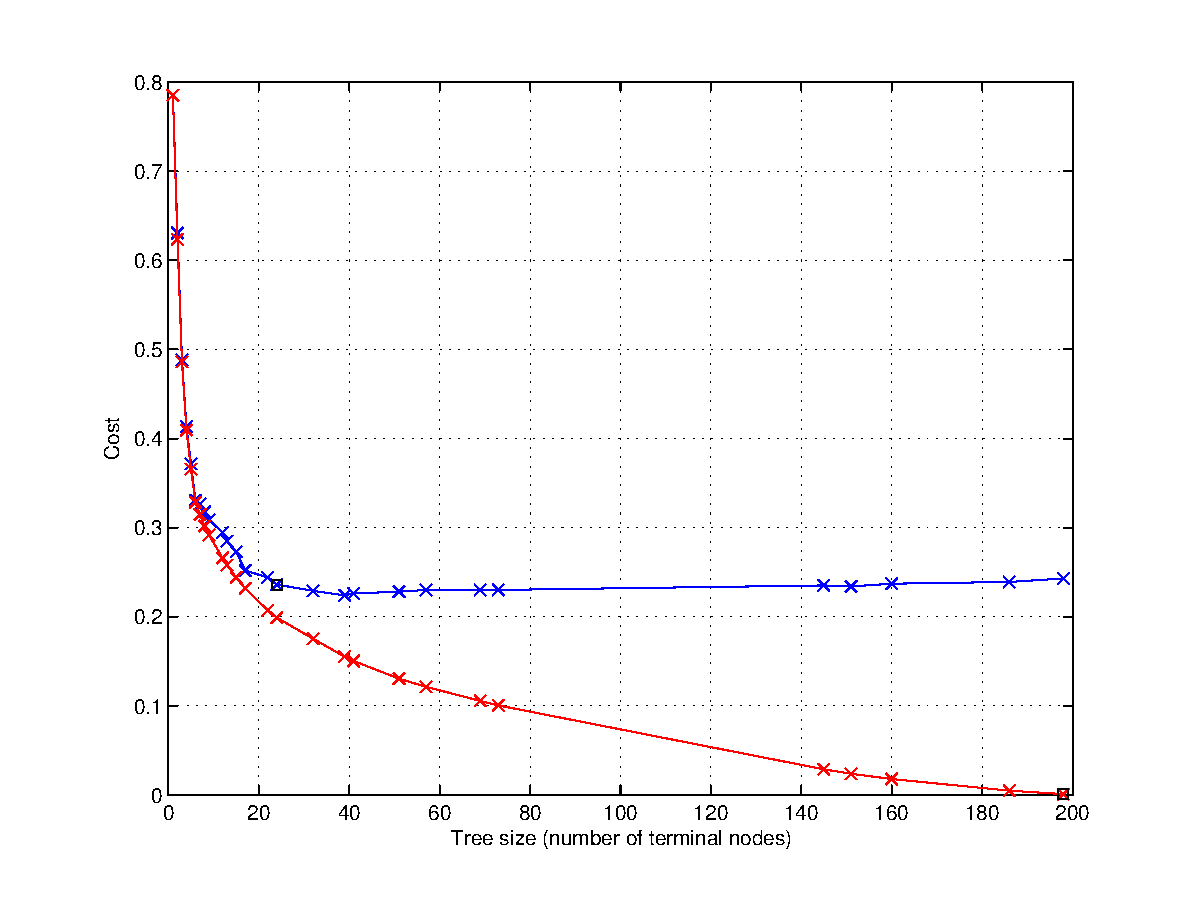
\includegraphics[width=\textwidth]{images/pruning_clean_data.eps}
     	\caption{Pruning Function Applied to Clean Data}
     	\label{fig:pruningClean}
    \end{subfigure}
	\begin{subfigure}[b]{0.495\textwidth}
		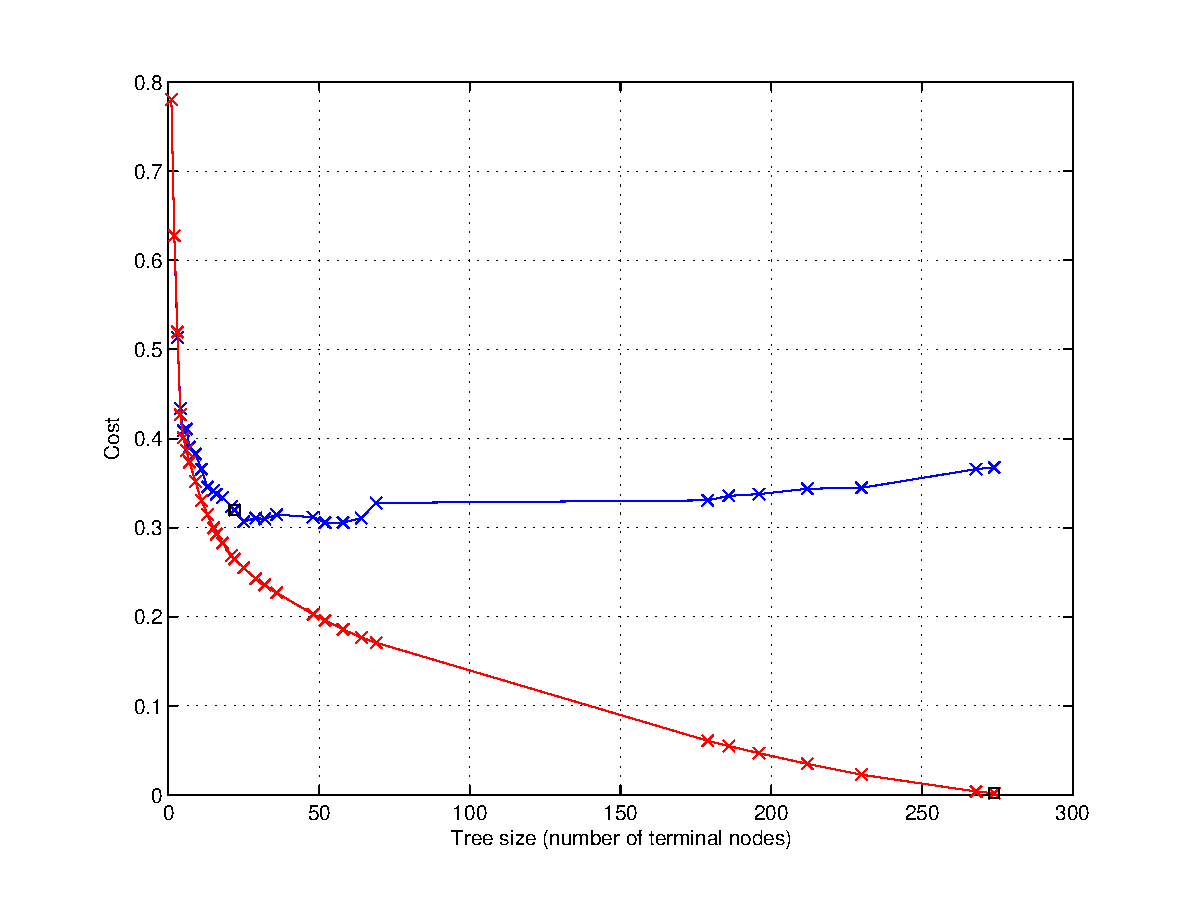
\includegraphics[width=\textwidth]{images/pruning_noisy_data.eps}
     	\caption{Pruning Function Applied to Noisy Data}
     	\label{fig:pruningNoisy}
    \end{subfigure}
    \caption{Tree Pruning Example}
    \label{fig:pruning}
\end{figure}

As we can see in the graphs, the curves corresponding to clean data (figure \ref{fig:pruningClean}) drop faster than the other curves. This is caused by the lack of inconsistencies in the data which means that classification is only hindered by absence of knowledge rather than also conflicting parts of knowledge. Notice that this also has a much larger effect on the development of the verification error rate in figure \ref{fig:pruningNoisy} that corresponds to the noisy data. In noisy (and more likely real-life data) it is thus very important not to overfit the classifier.
% rewrite this a bit?

\begin{figure}[!hb]
	\centering
	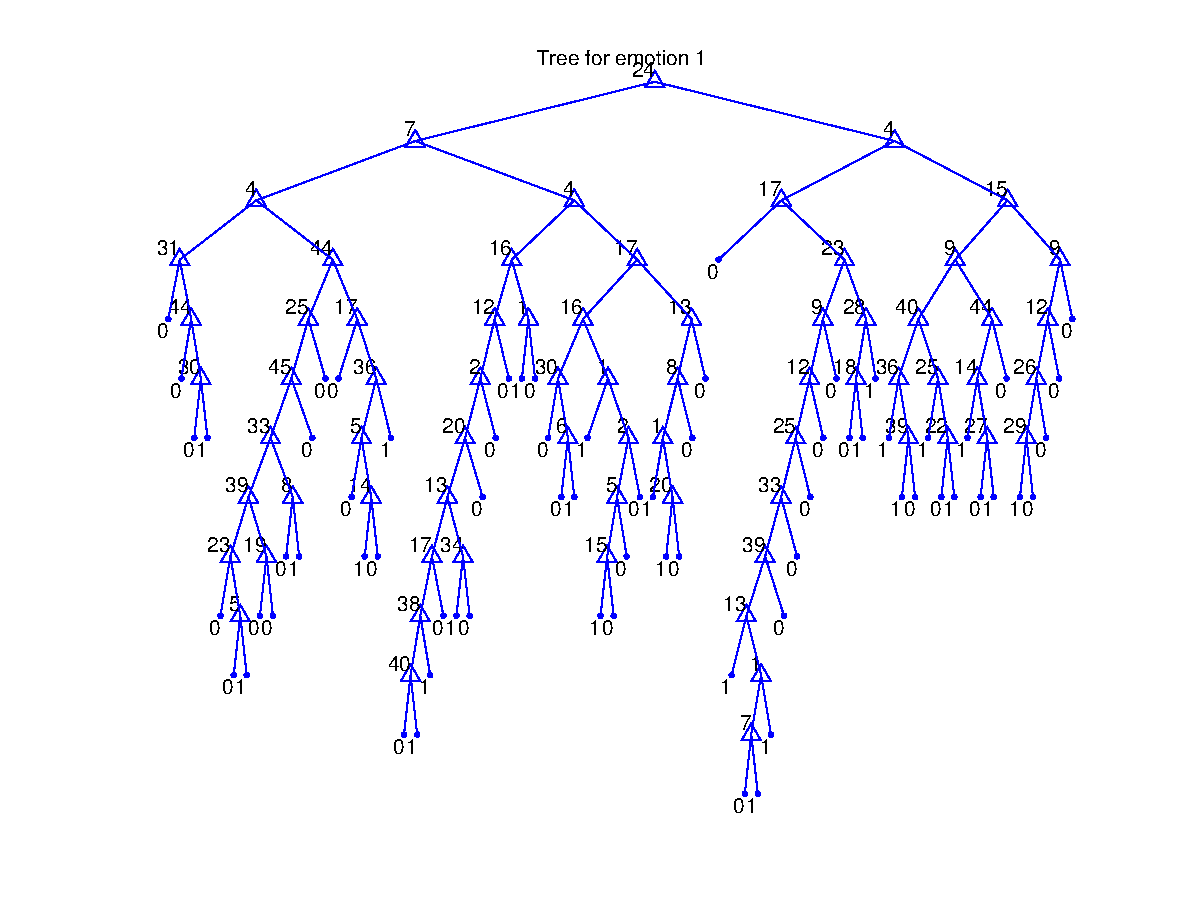
\includegraphics[width=\textwidth]{trees/tree1.eps}
     \caption{Tree For Emotion 1}
     \label{fig:tree1}
\end{figure}
\begin{figure}[!ht]
	\centering
	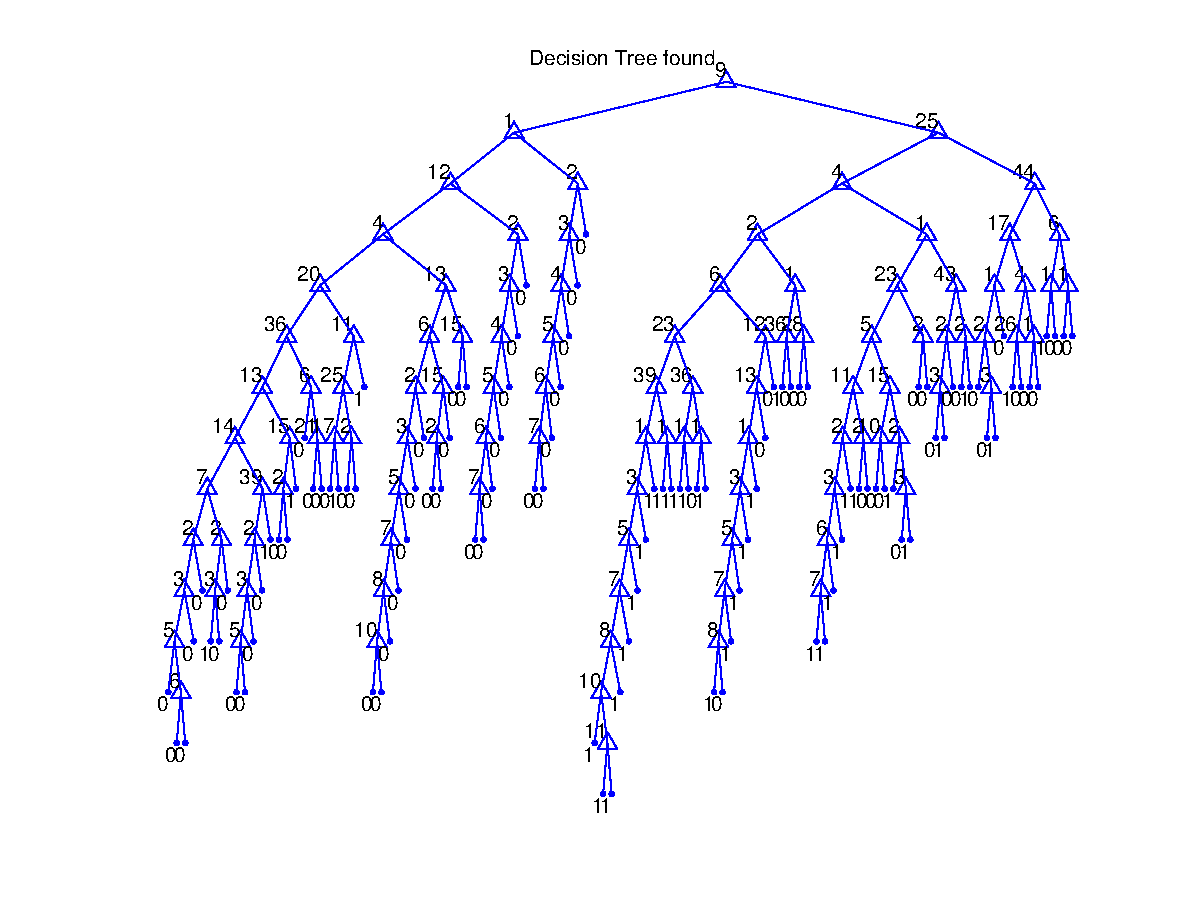
\includegraphics[width=\textwidth]{trees/tree2.eps}
     \caption{Tree For Emotion 2}
     \label{fig:tree2}
\end{figure}
\begin{figure}[!hb]
	\centering
	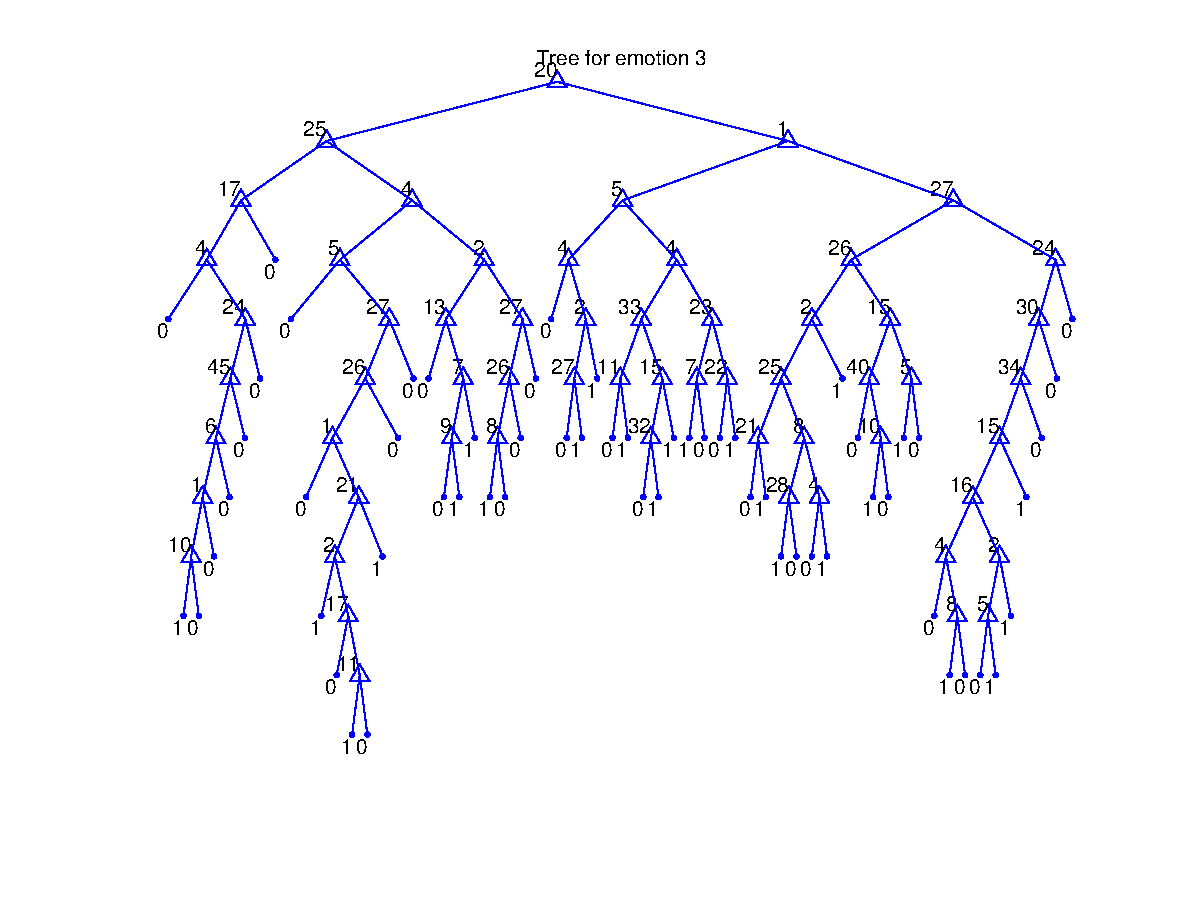
\includegraphics[width=\textwidth]{trees/tree3.eps}
     \caption{Tree For Emotion 3}
     \label{fig:tree3}
\end{figure}
\begin{figure}[!ht]
	\centering
	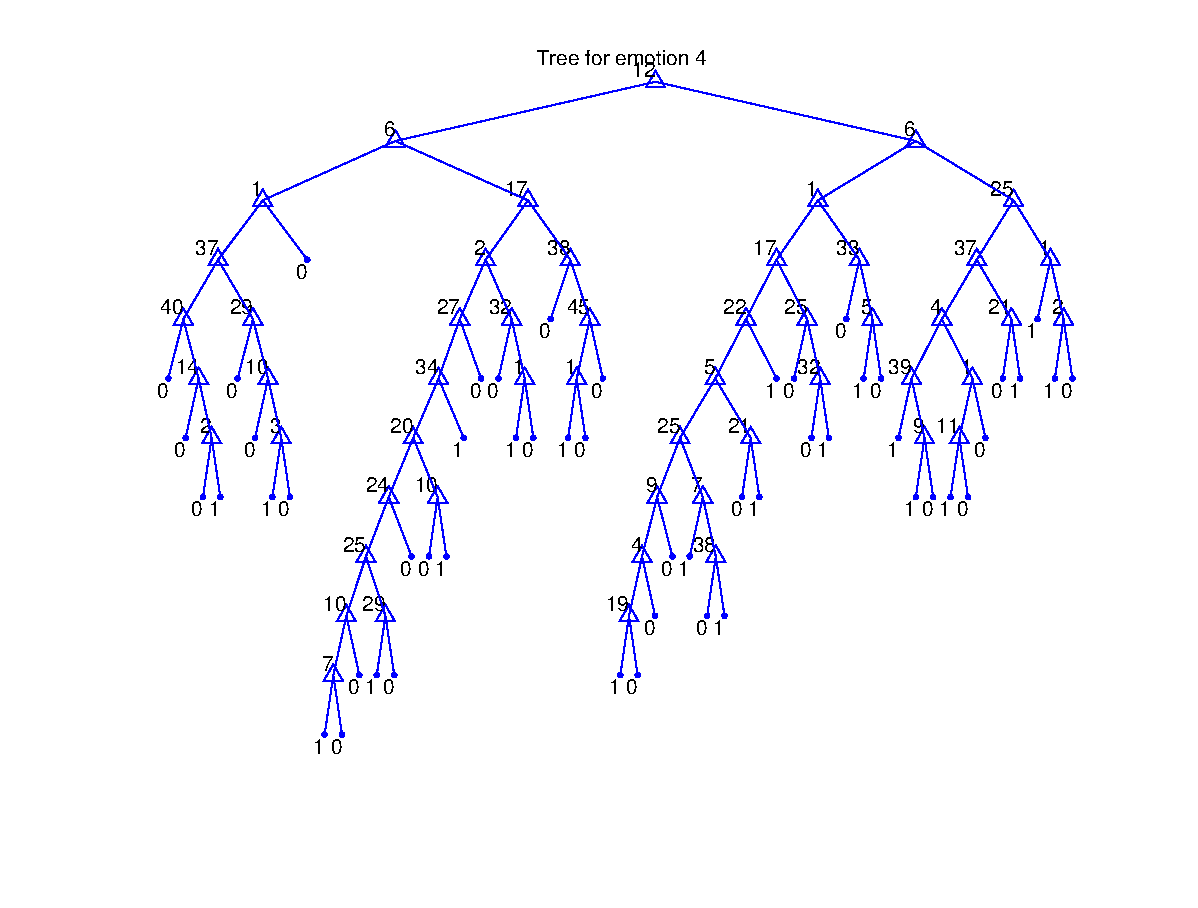
\includegraphics[width=\textwidth]{trees/tree4.eps}
     \caption{Tree For Emotion 4}
     \label{fig:tree4}
\end{figure}
\begin{figure}[!hb]
	\centering
	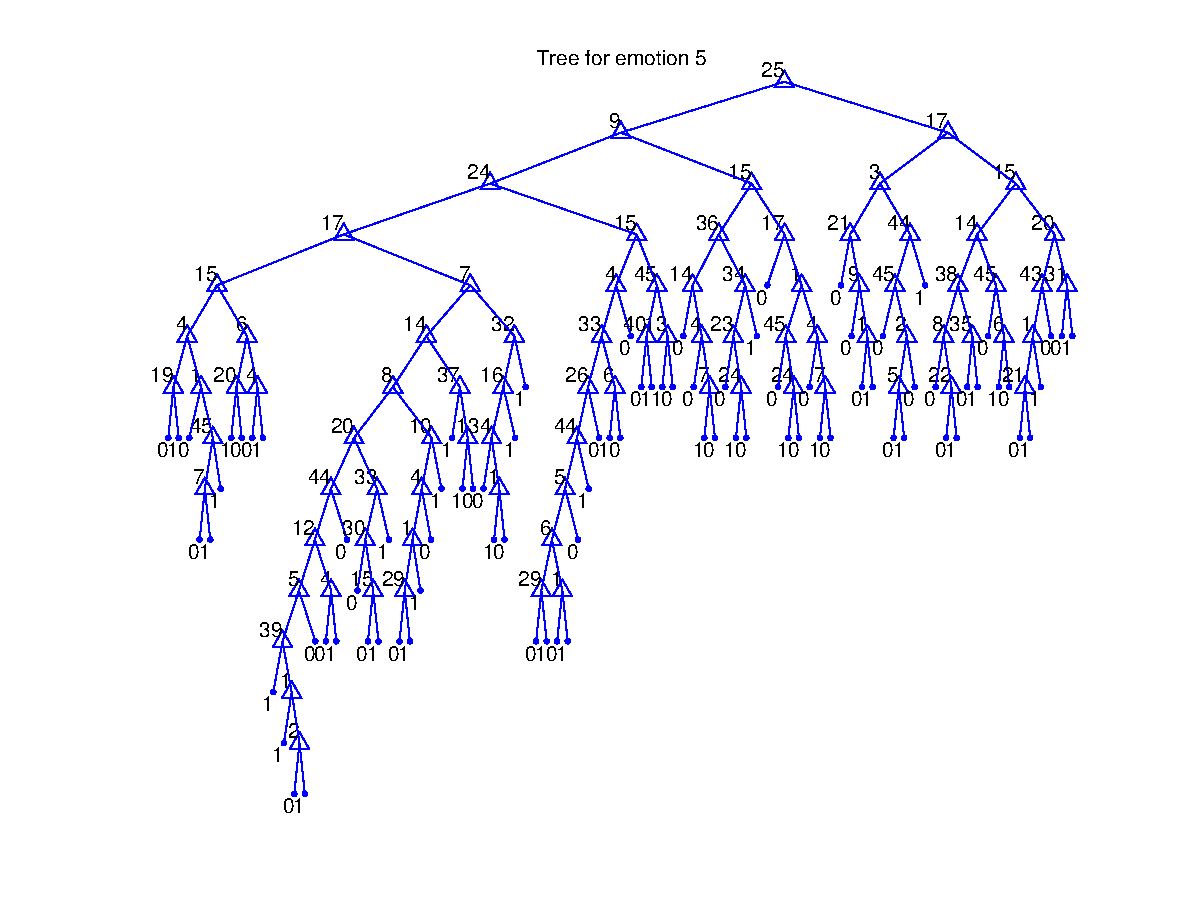
\includegraphics[width=\textwidth]{trees/tree5.eps}
     \caption{Tree For Emotion 5}
     \label{fig:tree5}
\end{figure}
\begin{figure}[!ht]
	\centering
	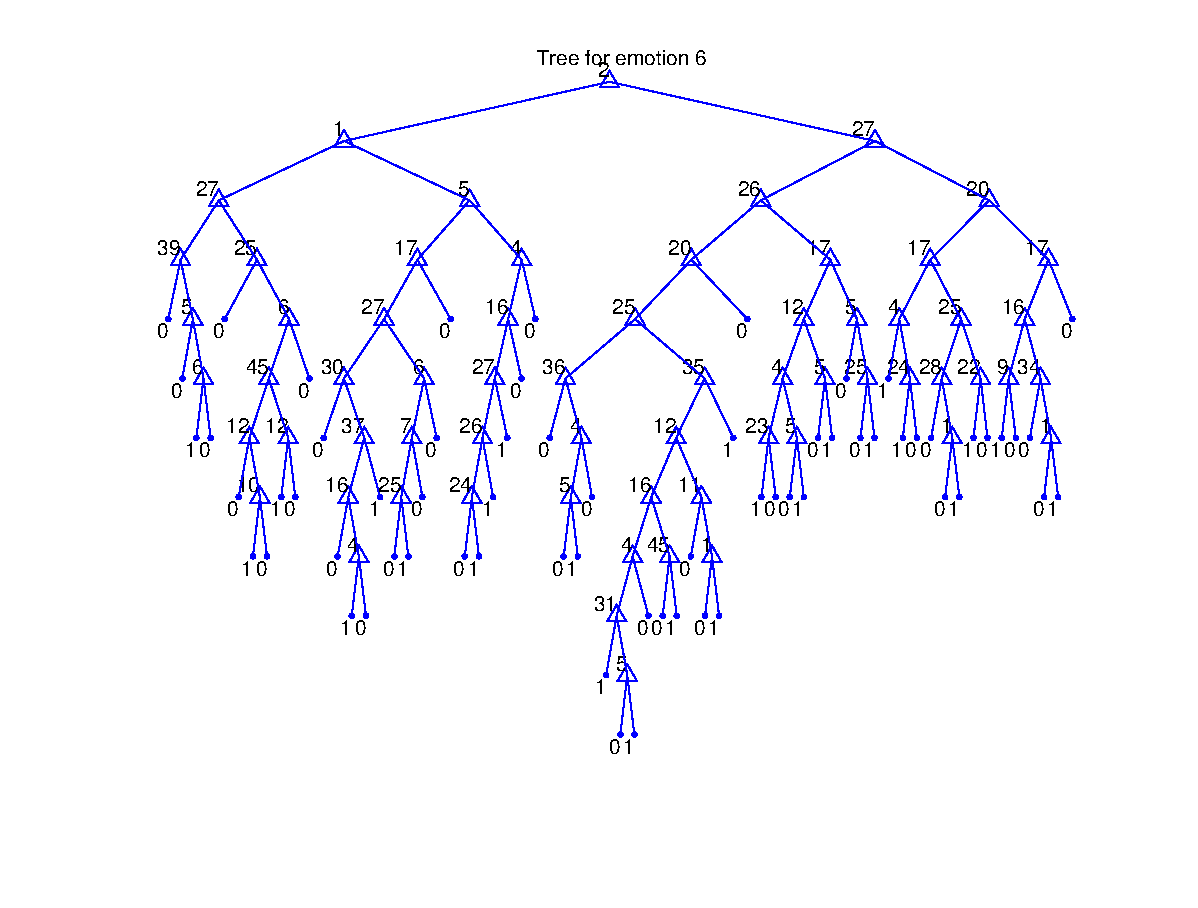
\includegraphics[width=\textwidth]{trees/tree6.eps}
     \caption{Tree For Emotion 6}
     \label{fig:tree6}
\end{figure}

\section{Flowcharts}
See Figure~\ref{fig:cross_fold_validation} for function {\tt cross\_fold\_validation}, Figure~\ref{fig:create_folds} for function {\tt create\_folds}, Figure~\ref{fig:build_tree} for function {\tt build\_tree}, 
Figure~\ref{fig:binary_filter} for function {\tt binary\_filter}, Figure~\ref{fig:id3} for function {\tt decision\_tree\_learning}, Figure~\ref{fig:choose_best_decision_attribute} for function {\tt choose\_best\_decision\_attribute},
Figure~\ref{fig:entropy} for function {\tt I}, Figure~\ref{fig:remainder} for function {\tt remainder}, Figure~\ref{fig:test_trees} for function {\tt test\_trees}, and Figure~\ref{fig:test_tree} for function {\tt test\_tree}.


\begin{figure}[!ht]
	\centering
	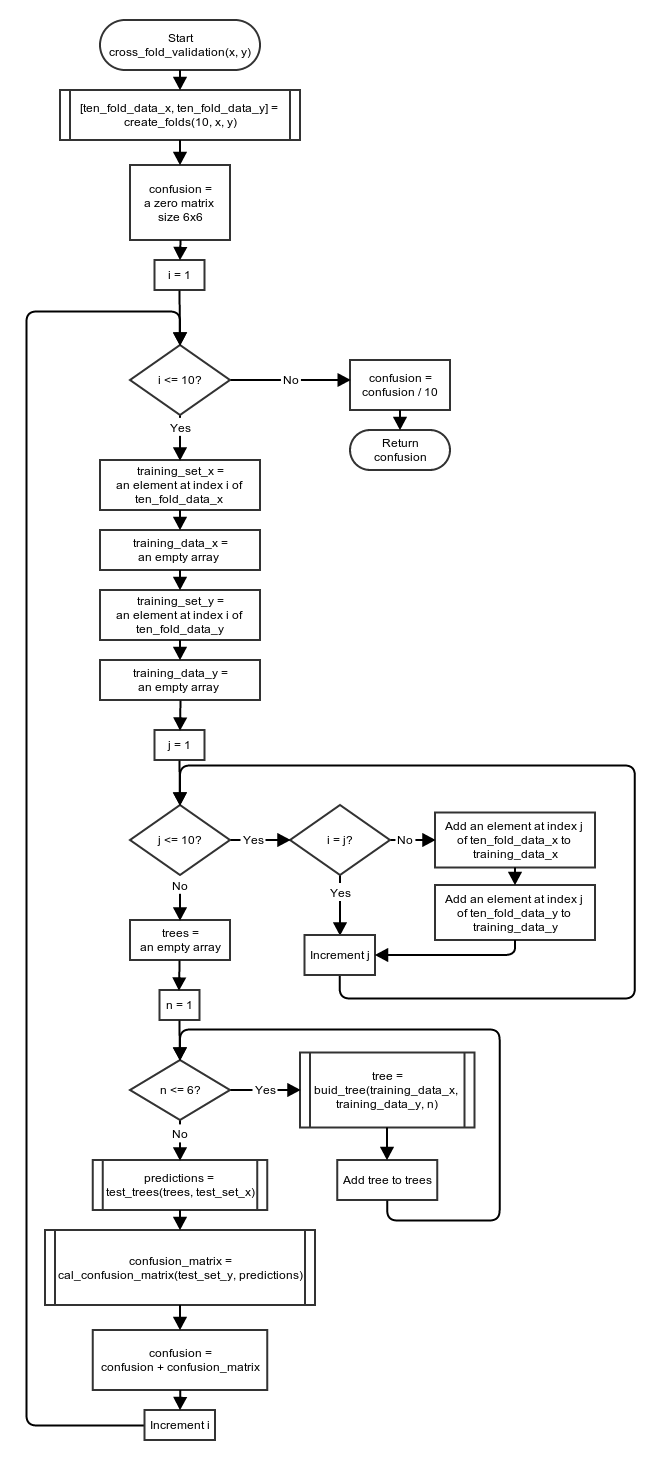
\includegraphics[width=0.65\textwidth]{images/flow_chart/cross_fold_validation.png}
	\caption{Flowchart of \tt{cross\_fold\_validation}}
	\label{fig:cross_fold_validation}
\end{figure}

\begin{figure}[!ht]
	\centering
	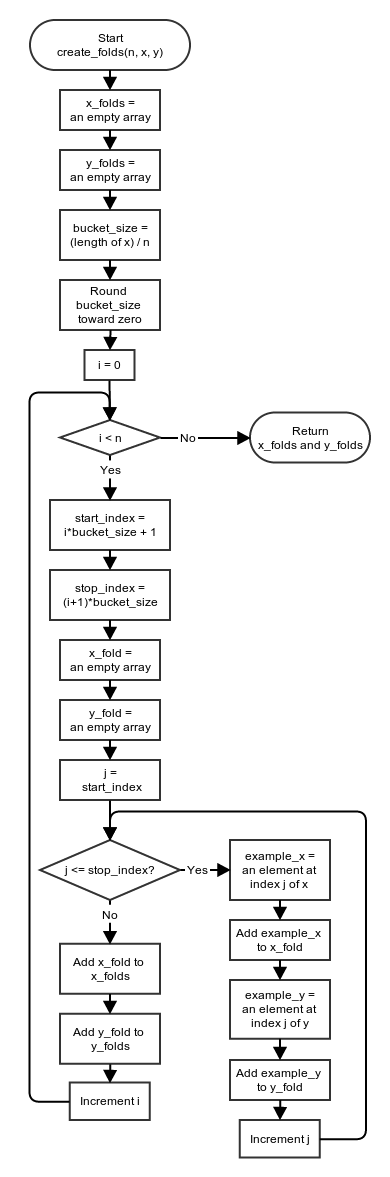
\includegraphics[scale=0.54]{images/flow_chart/create_folds.png}
	\caption{Flowchart of \tt{creat\_folds}}
	\label{fig:create_folds}
\end{figure}

\begin{figure}[!ht]
	\centering
	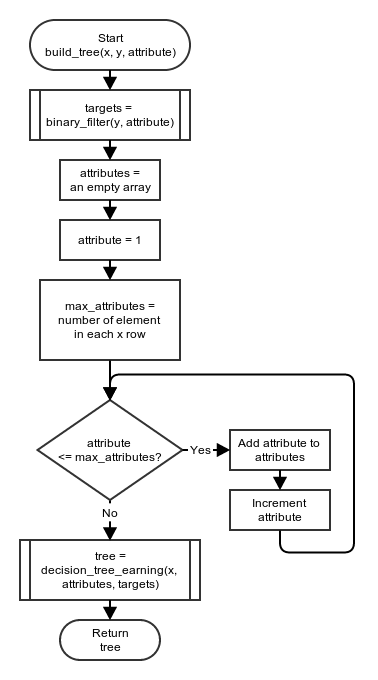
\includegraphics[scale=0.56]{images/flow_chart/build_tree.png}
	\caption{Flowchart of \tt{build\_tree}}
	\label{fig:build_tree}
\end{figure}

\begin{figure}[!ht]
	\centering
	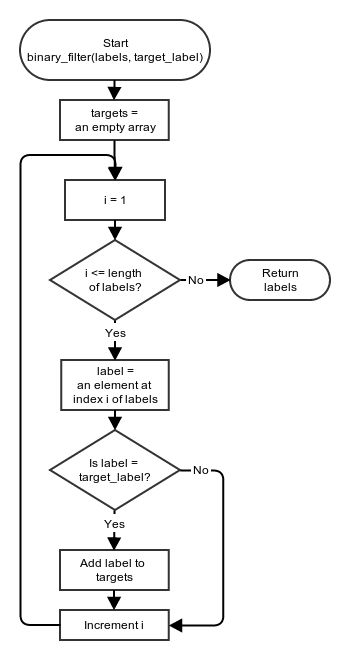
\includegraphics[scale=0.66]{images/flow_chart/binary_filter.png}
	\caption{Flowchart of \tt{binary\_filter}}
	\label{fig:binary_filter}
\end{figure}

\begin{figure}[!ht]
	\centering
	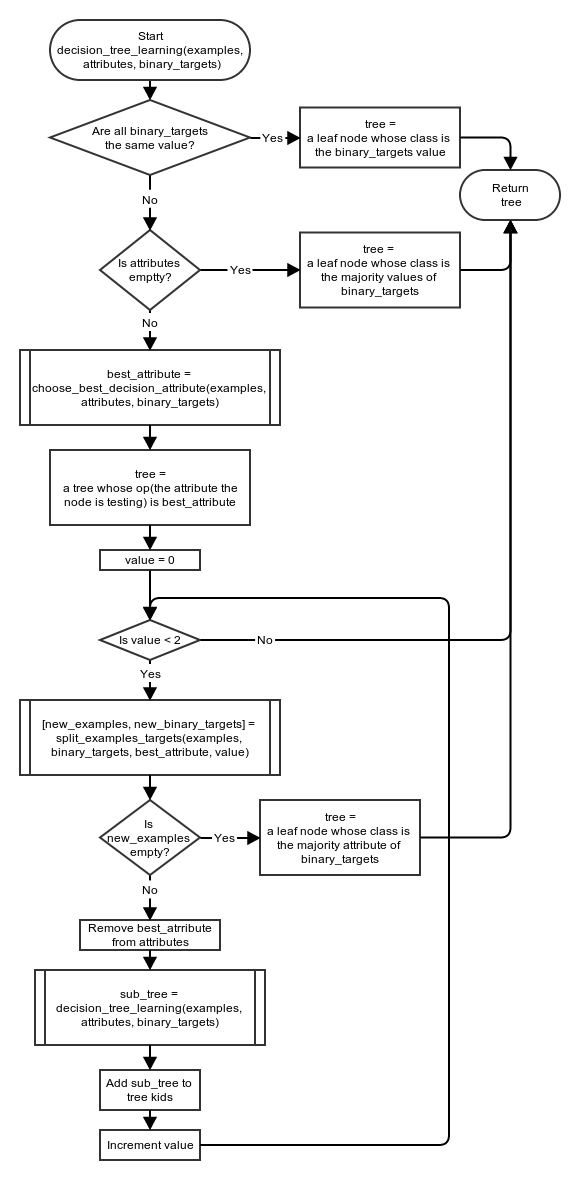
\includegraphics[scale=0.56]{images/flow_chart/id3.png}
	\caption{Flowchart of \tt{decision\_tree\_learning}}
	\label{fig:id3}
\end{figure}


\begin{figure}[!ht]
	\centering
	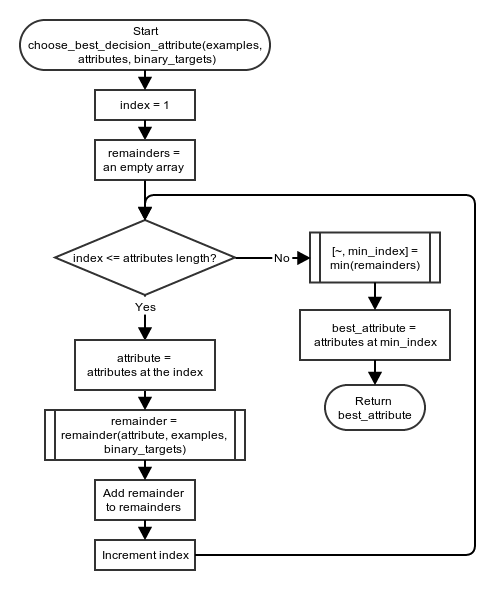
\includegraphics[height=15cm, width=10cm]{images/flow_chart/choose_best_decision_attribute.png}
	\caption{Flowchart of \tt{choose\_best\_decision\_attribute}}
	\label{fig:choose_best_decision_attribute}
\end{figure}

\begin{figure}[!ht]
	\centering
	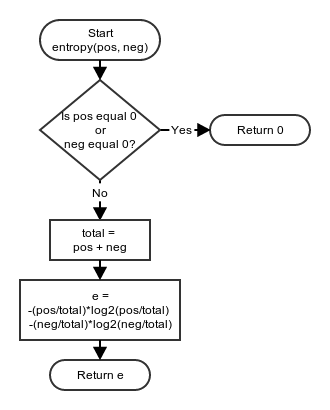
\includegraphics[height=7cm, width=8cm]{images/flow_chart/entropy.png}
	\caption{Flowchart of \tt{entropy}}
	\label{fig:entropy}
\end{figure}

\begin{figure}[!ht]
	\centering
	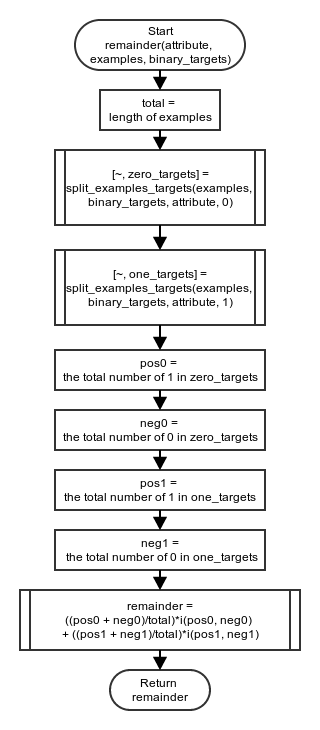
\includegraphics[width=8cm]{images/flow_chart/remainder.png}
	\caption{Flowchart of \tt{remainder}}
	\label{fig:remainder}
\end{figure}

\begin{figure}[!ht]
	\centering
	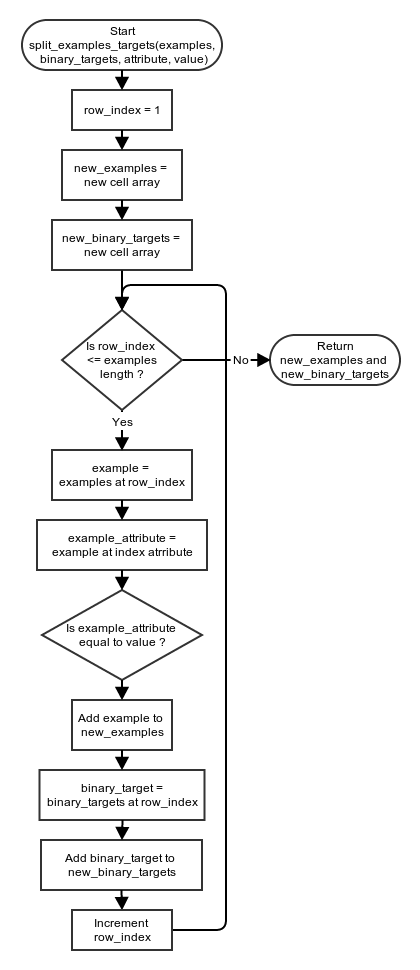
\includegraphics[height=0.9\textheight]{images/flow_chart/split_examples_targets.png}
	\caption{Flowchart of \tt{split\_examples\_targets}}
	\label{fig:split_examples_targets}
\end{figure}

\begin{figure}[!ht]
	\centering
	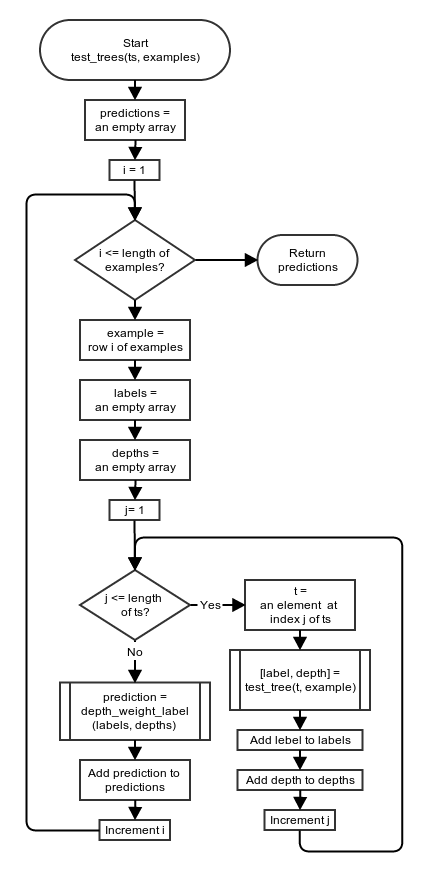
\includegraphics[scale=0.6]{images/flow_chart/test_trees.png}
	\caption{Flowchart of \tt{test\_trees}}
	\label{fig:test_trees}
\end{figure}

\begin{figure}[!ht]
	\centering
	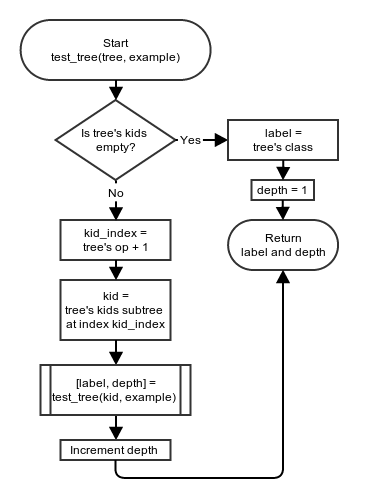
\includegraphics[height=15cm, width=10cm]{images/flow_chart/test_tree.png}
	\caption{Flowchart of \tt{test\_tree}}
	\label{fig:test_tree}
\end{figure}

\begin{figure}[!ht]
	\centering
	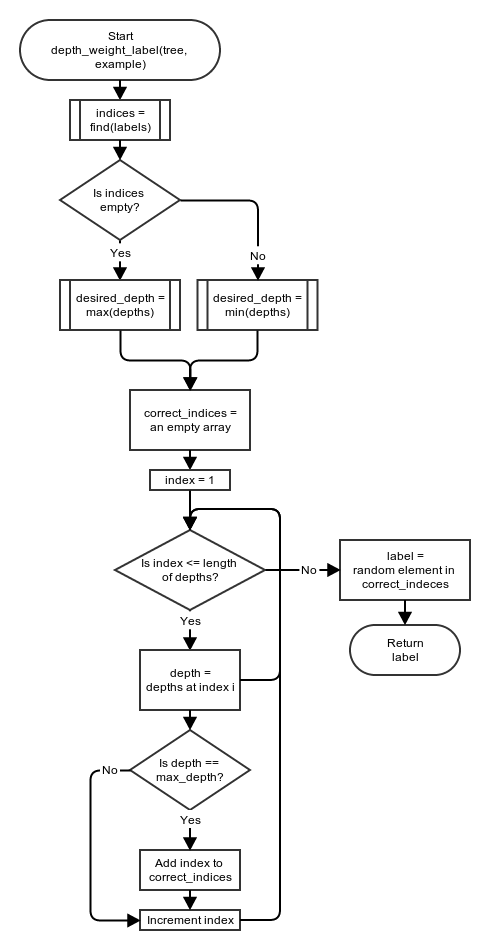
\includegraphics[height=20cm, width=10cm]{images/flow_chart/depth_weight_label.png}
	\caption{Flowchart of \tt{depth\_weight\_label}}
	\label{fig:depth_weight_label}
\end{figure}

\begin{figure}[!ht]
	\centering
	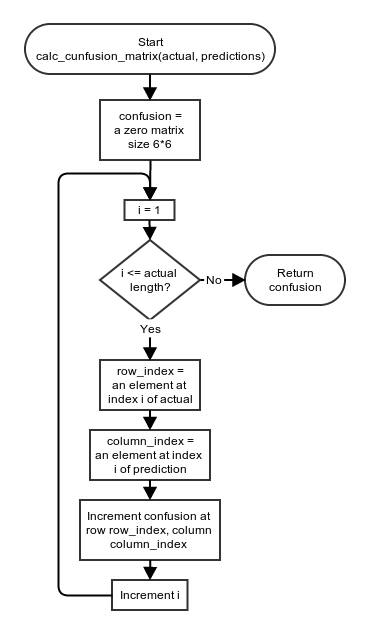
\includegraphics[height=15cm, width=10cm]{images/flow_chart/calc_confusion_matrix.png}
	\caption{Flowchart of \tt{calc\_confusion\_matrix}}
	\label{fig:calc_confusion_matrix}
\end{figure}

\end{document}
